\documentclass[final]{beamer}
\mode<presentation>
{
  \usetheme{I6pd2}
}
\graphicspath{{figures/}} % e.g. where you have your logos

\usepackage{times}
\usepackage{amsmath,amssymb}
\usepackage[english]{babel}
%\usepackage[latin1]{inputenc}
\usepackage[orientation=portrait,size=a0,scale=1.4,debug]{beamerposter} 
\usepackage{xcolor}
\definecolor{JungleGreen}{RGB}{188,210,238}
\definecolor{MedGrey}{RGB}{201,201,201}


\title[Fancy Posters]{High-Order Rogue Waves in the Nonlinear Schr\"{o}dinger Equation}
\subtitle[]{\textit{Physical Sciences, Mathematics \& Engineering}}
\author[]{Andrew Reagan, 2013}
\institute[]{Christopher M. Danforth \& Jianke Yang, College of Engineering \& Mathematical Sciences}
\date{\today}

\begin{document}
\begin{frame}{} 

\vspace{-1cm}

\begin{columns}[t]

\begin{column}{.005\linewidth}
\end{column}

	\begin{column}{.35\linewidth}
%    \setbeamercolor{block title}{bg=black, fg=tabutter}
%		\setbeamercolor{block body}{bg=ta3aluminium, fg=black}
	\begin{block}{Introduction}
	In oceanography, the pragmatic approach is to define a rogue wave whenever
\[ H/H_s > 2 ~\text{or} ~ c/H_s > 1.25 \]
where $H$ is the wave height (distance from trough to crest), $c$ is the crest height (distance from mean sea level to crest), and $H_s$ is the significant wave height, here defined as four times the standard deviation of the surface elevation.\\
	\vspace{5mm}
	The ``Draupner Wave" was the first recorded:
	
	\centering
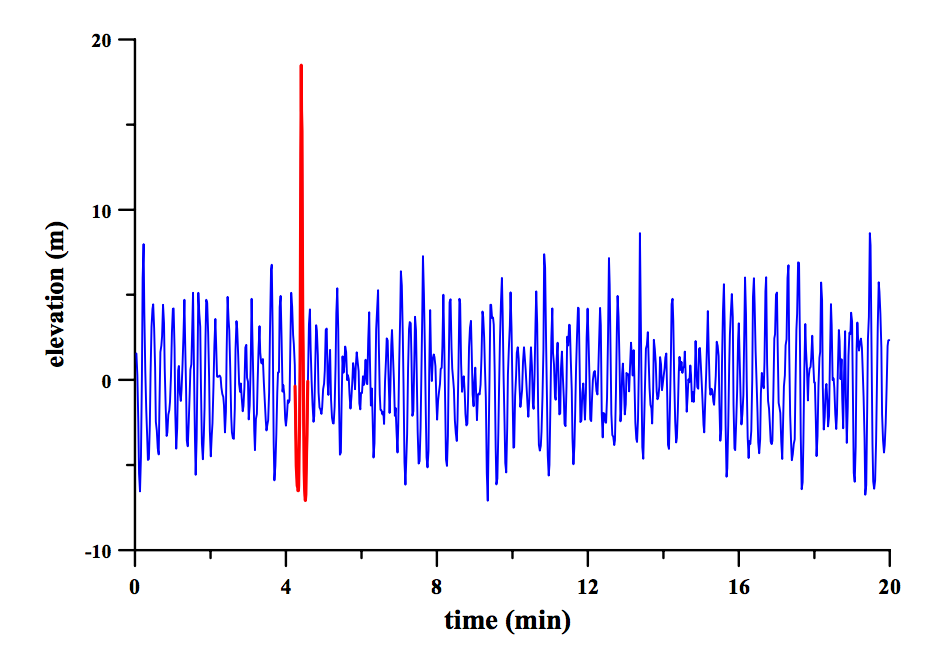
\includegraphics[width=600px]{draupner_wave.png}
	\end{block}
	\hspace{0.25cm}
	\begin{block}{Methods/Data}
The Focusing Nonlinear Schr\"{o}dinger Equation (NSE) has been derived as a general nonlinear wave equation, in particular describing deep water waves. The focusing equation is written as: \[ i\frac{\partial u}{\partial t} + \frac{\partial ^2 u}{\partial x^2} + 2 |u| ^2 u = 0 .\] Ohta and Yang (2012) found rational solutions with rogue-wave characteristics, first described by Peregrine in 1983 as a result of modulation instability. These solutions are part of a hierarchy of solutions that exhibit large peaks that seemingly emerge from a constant background for finite time, then disappear in the same way.\\
\vspace{5mm}
Using an innovative combination of MATLAB and Mathematica scripts, we are able to simulate higher order waves than otherwise possible.
	\end{block}
	\hspace{0.25cm}
  	\begin{block}{Results}
For a specific choice of the free parameters in the 3rd order solution, we generate waves in space-time as below:

\vspace{3cm}
\centering
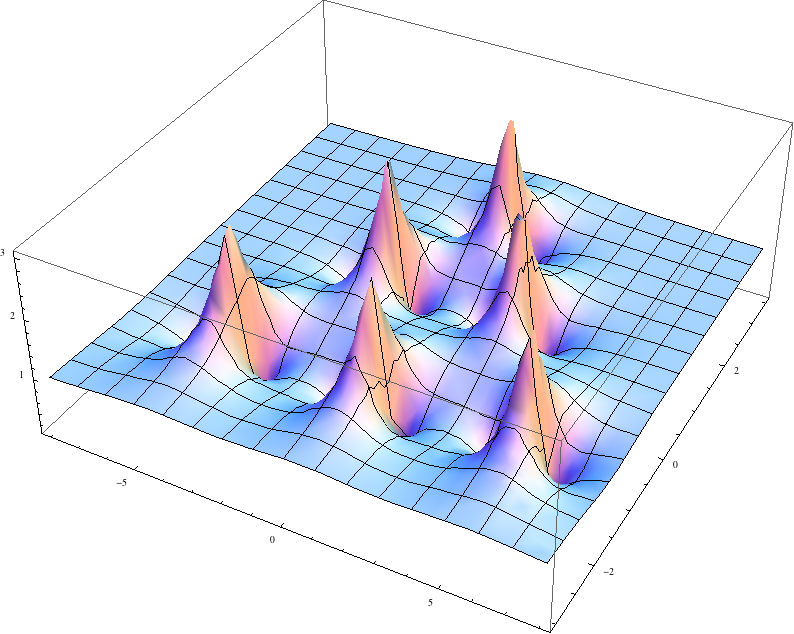
\includegraphics[width=700px]{3rd_order_many_peaks.png}
\\[1ex]

		\end{block}
		  \setbeamercolor{block title}{bg=white, fg=white}
		\setbeamercolor{block body}{bg=white, fg=white}
	
\vspace{1cm}
  		
  		
\includegraphics[width=1\linewidth]{SSPC_logo.pdf}

	\end{column}
	
	\begin{column}{.005\linewidth}	
\end{column}  

\begin{column}{.35\linewidth}
%      \setbeamercolor{block title}{bg=black, fg=tabutter}
%		\setbeamercolor{block body}{bg=ta3aluminium, fg=black}
\begin{block}{Resolving Numerical Instability}
	Due to the size of the rational solution, a naive approach to visualizing the solution is futile. The instability can be seen in the red regions below:
	
	\centering 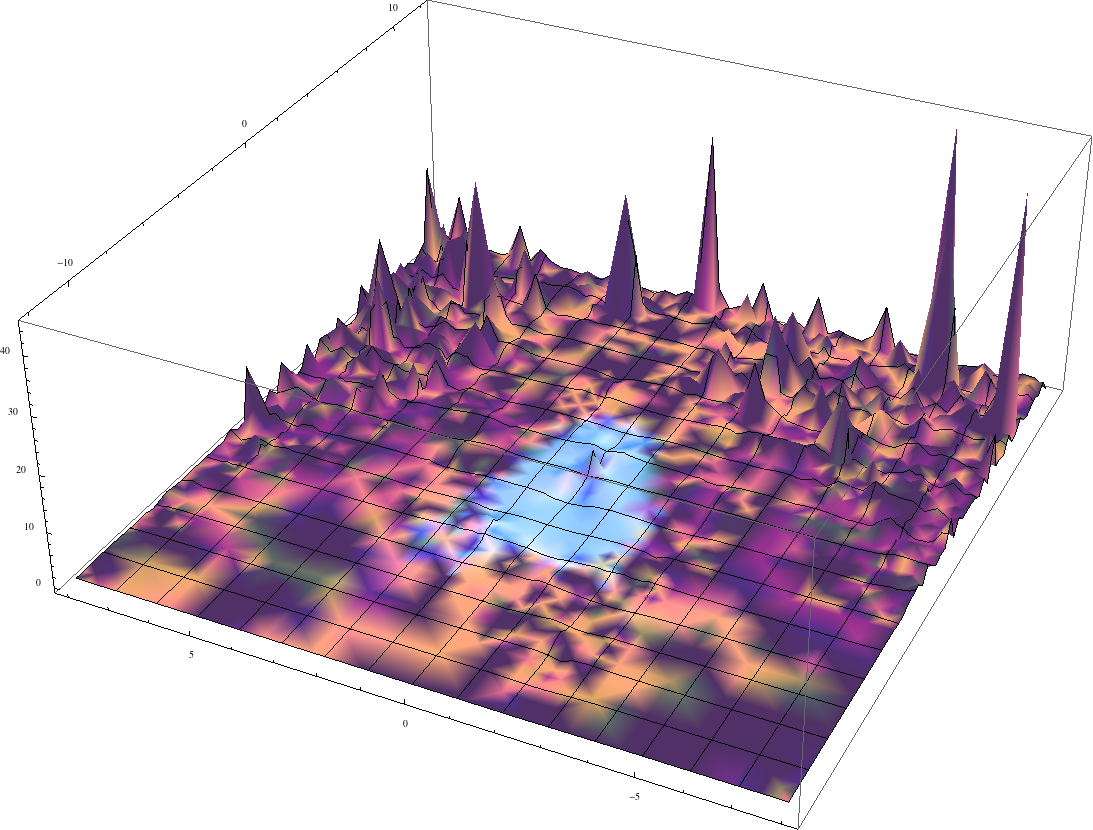
\includegraphics[width=600px]{5th_order_unstable.png} \\[1ex]
	
	
		\begin{flushleft} Capitalizing on Mathematica's symbolic capability, and MATLAB's plotting accuracy, we are able to see this 5th order wave: \end{flushleft}
			\centering
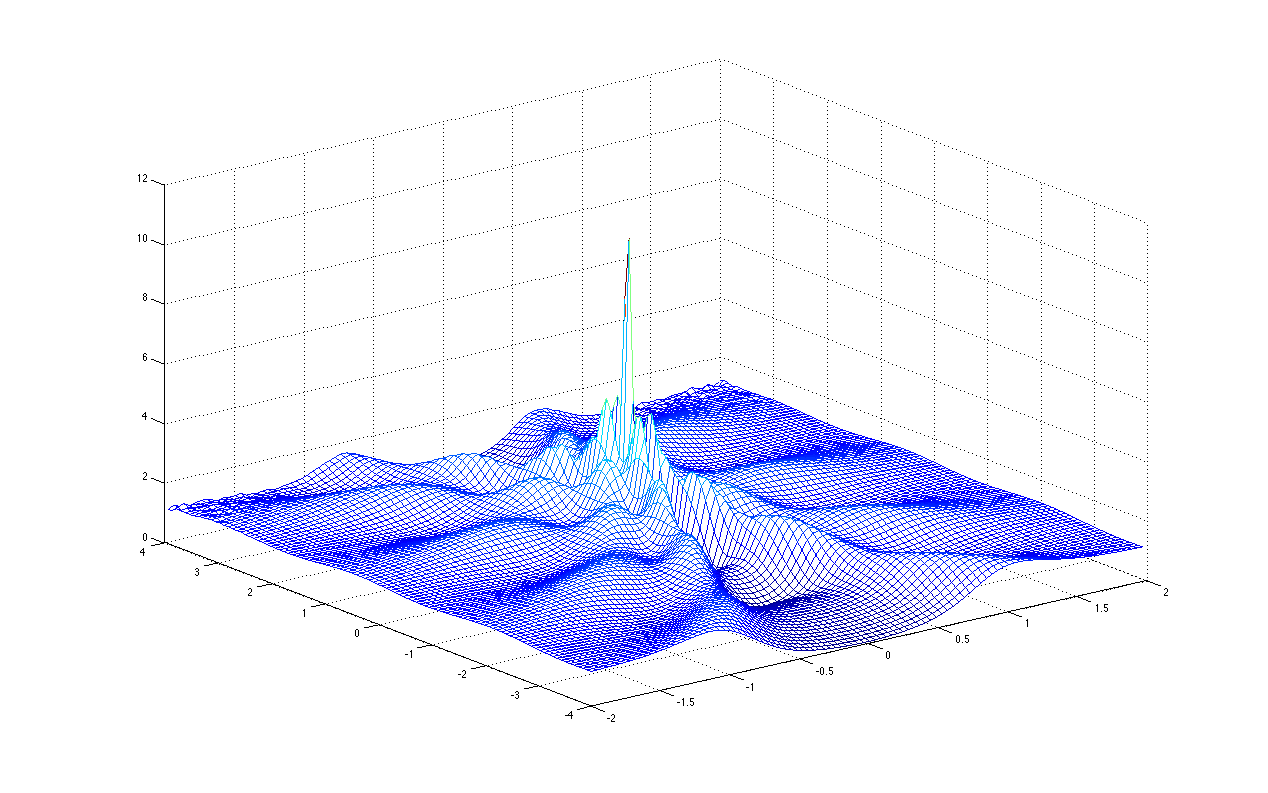
\includegraphics[width=670px]{matlab_5th_order_peak.png}
		\\[1ex]
		
		\vspace{-1cm}
		\end{block}
			\hspace{0.25cm}

		\vspace{-.75cm}
		\begin{block}{Rogue Waves from Modulation Instability}
	The Benjamin-Feir instability of the NSE shows the system is ill posed as an initial value problem with the initial data  in the form of a modulated plane wave. As a result, this plane wave is expected to break immediately into some other, presumably disordered, wave form.\\
	
	\vspace{5mm}
In the case of an analytic initial data, the NLS evolution displays some ordered structure instead of the disorder suggested by the modulational instability. Below is a plot of the gradient catastrophe for \[ u=e^{-x^2}e^{-i\log (\cosh (x)) /\epsilon } \]
		
		\vspace{-.25cm}
				\centering
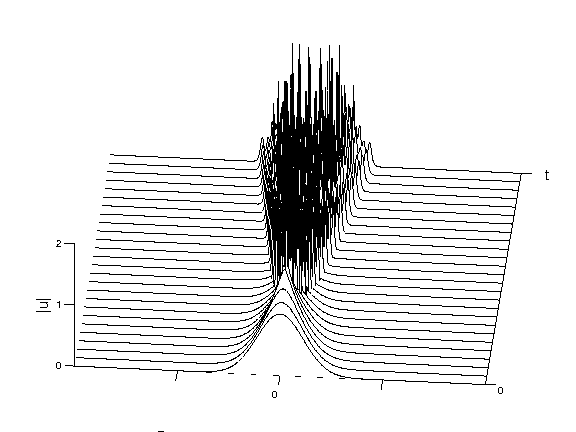
\includegraphics[width=670px]{t1_65536pts_512plotted.png}


			\end{block}
		\hspace{0.25cm}
			\begin{block}{Conclusions}
	Rogue waves do exist as solutions to the NSE. By analyzing their structure through simulations, more insight into the universal structure of their formation can be gained. With a better understanding of their structure, early warning systems and detection can make our seas safer. Further simulations will aim to quantify uncertainty from the structure of noisy initial conditions on the formation of large waves events.\\[1ex]
		\end{block}
		
		
\end{column}  


\begin{column}{.005\linewidth}
\end{column}  
	\begin{column}{.255\linewidth}
%	  \setbeamercolor{block title}{bg=black, fg=tabutter}
%		\setbeamercolor{block body}{bg=ta3aluminium, fg=black}
   
		\begin{block}{Project Description}

Once considered to be a mythical occurrence, rogue waves are now a studied phenomenon in nonlinear wave theory. The structure and nature of these waves is imperative in our understanding of how and why they occur. Their occurrence in both water and optical waves, although neither periodic nor obvious, has an affect on our everyday lives. They are known to cause extensive damage, and are even life-threatening, when they come into contact with ocean liners and passenger ships in the open waters. Between 1964 and 1994, it is estimated that more than 22 super-carriers have been lost at sea as a direct result of rogue waves. The importance of these waves goes beyond water, to optical systems, where it would be valuable to be able to predict the initial conditions of the light pulse so as to produce extreme intensity pulses at well-determined positions and time steps.\\

\vspace{0.5cm}
We summarize our work as follows:\\
		
		\vspace{.5cm}
(1) We simulated higher order waves than previously possible.\\

			\vspace{.5cm}
(2) By studying the structure of the gradient catastrophe due to modulation instability in relation to rogue wave, we predict the spatial distribution of these waves.\\

			\vspace{.5cm}	
(3) A better understanding of the nonlinear effects that lead to rogue wave formation will be essential in the develop of techniques for early warning, with great safety and economic importance.\\

\vspace{1cm}
\end{block}
\vspace{1cm}
	\begin{block}{Acknowledgments}
	

{\small References:}\\

{\footnotesize Ohta, Y. \& Yang, J. 2012 General rogue waves in the NLS equation. The Royal Society. (doi: 10.1098/rspa.20110640)}\\

{\footnotesize Peregrine, D.H. 1983 Water waves, nonlinear Schr\"{o}dinger equations and their solutions. J. Aust. Math. Soc. B 25, 16-43. (doi:10.1017/S0334270000003891)}
	
\vspace{2cm}
	{\small This work was supported in part by NASA, the National Science Foundation, and the Vermont Advanced Computing Core.}\\
\vspace{1cm}	
			\centering
	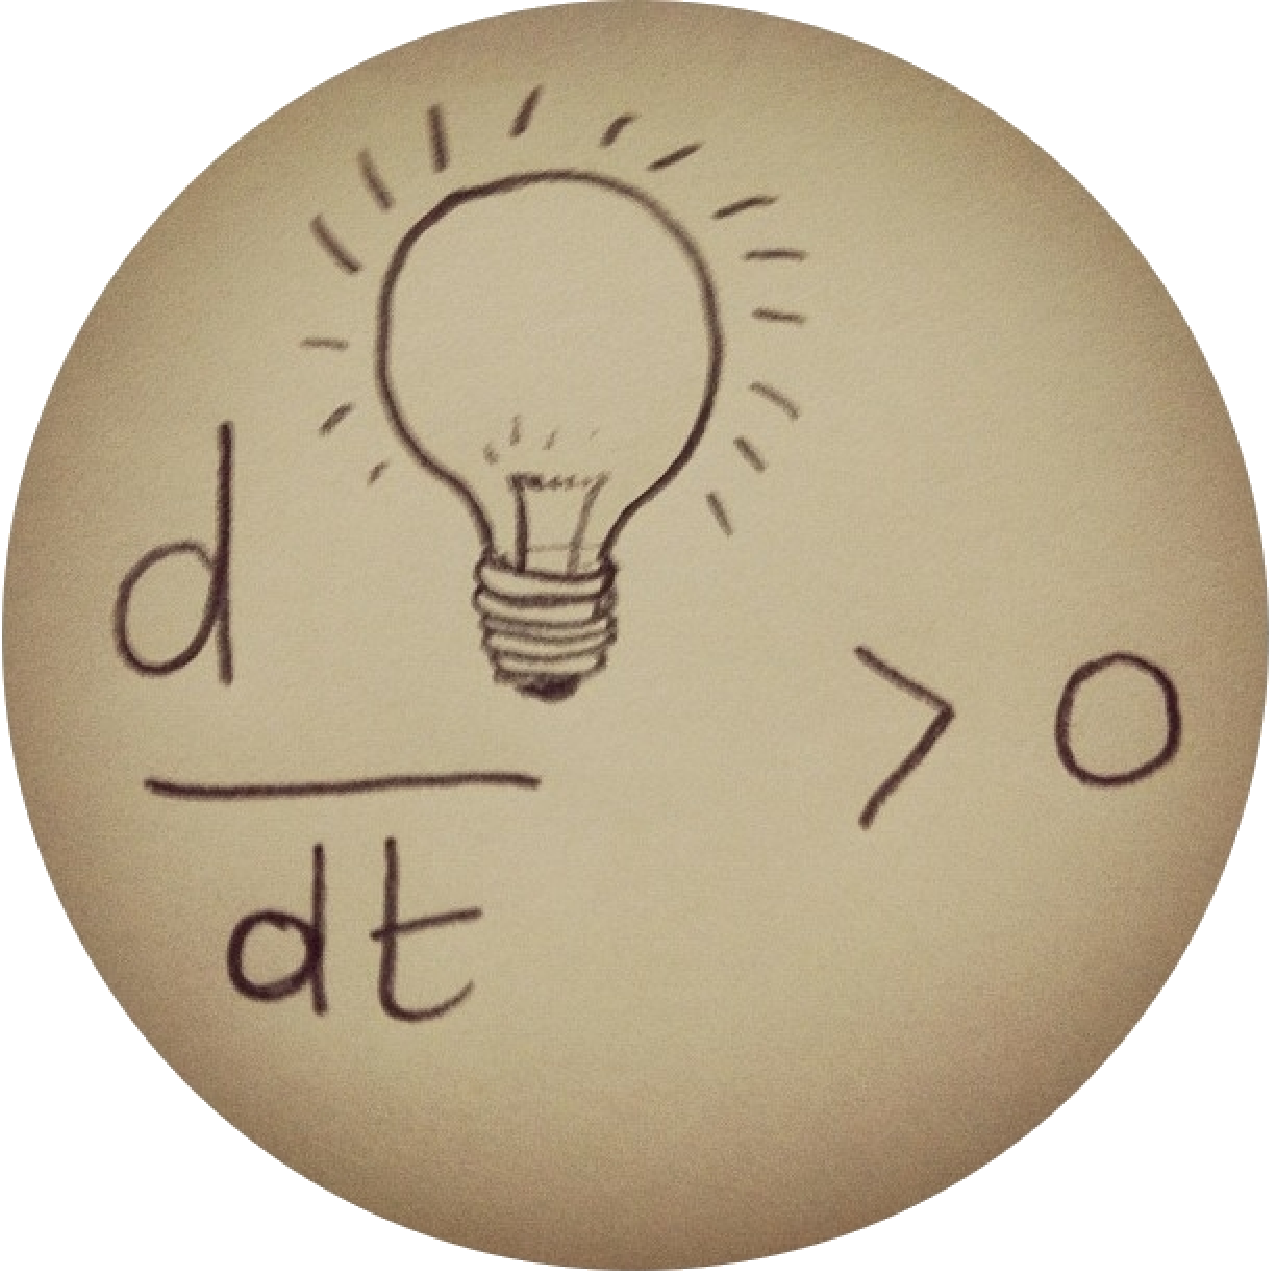
\includegraphics[width=.35\linewidth]{lightbulb-idea-calculus-circle-tp-1.pdf}
\hspace{.3cm}
  		  		
\includegraphics[width=.4\linewidth]{nsf-logo-tp-10.pdf}\\
  		  		
				
				
\includegraphics[width=.4\linewidth]{logo_VACC_logo_huge-tp.pdf}
  		  		\hspace{.3cm}
  		  		
\includegraphics[width=.4\linewidth]{logo_CSC_logo_cropped-tp.pdf}
				
  		\vspace{.5cm}
		\end{block}
		

	\end{column}
\begin{column}{.005\linewidth}
\end{column}  
  
  
\end{columns}

\end{frame}

\end{document}



